\chapter{PANGEOMETRY}

\section{Propositions Depending Only on the Principle of
Superposition}

\begin{description}
\item[1.~Theorem.] \emph{If one straight line meets another, the
sum of the adjacent angles formed is equal to two right angles.}

\item[2.~Theorem.] \emph{If two straight lines intersect, the
vertical angles are equal.}

\item[3.~Theorem.] \emph{Two triangles are equal if they have a
side and two adjacent angles, or two sides and the included angle,
of one equal, respectively, to the corresponding parts of the
other.}

\item[4.~Theorem.] \emph{In an isosceles triangle the angles
opposite the equal sides are equal.}

Bisect the angle at the vertex and use (3).

\item[5.~Theorem.] \emph{The perpendiculars erected at the middle
points of the sides of a triangle meet in a point if two of them
meet, and this point is the centre of a circle that can be drawn
through the three vertices of the triangle.}

\begin{figure}[h]
\centering
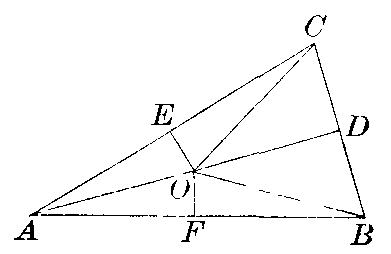
\includegraphics[width=40mm]{fig01.png}
\end{figure}

\textbf{Proof.} Suppose $EO$ and $FO$ meet at $O$. The triangles
$AFO$ and $BFO$ are equal by (3). Also, $AEO$ and $CEO$ are equal.
Hence, $CO$ and $BO$ are equal, being each equal to $AO$. The
triangle $BCO$ is, therefore, isosceles, and $OD$ if drawn bisecting
the angle $BOC$ will be perpendicular to $BC$ at its middle point.

\item[6.~Theorem.] \emph{In a circle the radius bisecting an angle at
the centre is perpendicular to the chord which subtends the angle
and bisects this chord.}

\item[7.~Theorem.] \emph{Angles at the centre of a circle are
proportional to the intercepted arcs and may be measured by them.}

\item[8.~Theorem.] \emph{From any point without a line a
perpendicular to the line can be drawn.}

\begin{figure}[h]
\centering
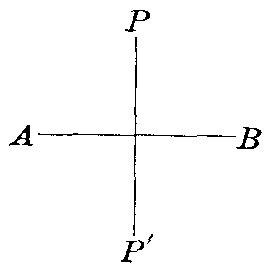
\includegraphics[width=20mm]{fig02.png}
\end{figure}

\textbf{Proof.} Let $P'$ be the position which $P$ would take if the
plane were revolved about $AB$ into coincidence with itself. The
straight line $PP'$ is then perpendicular to $AB$.

\item[9.~Theorem.] \emph{If oblique lines drawn from a point in a
perpendicular to a line cut off equal distances from the foot of the
perpendicular, they are equal and make equal angles with the line
and with the perpendicular.}

\begin{figure}[h]
\centering
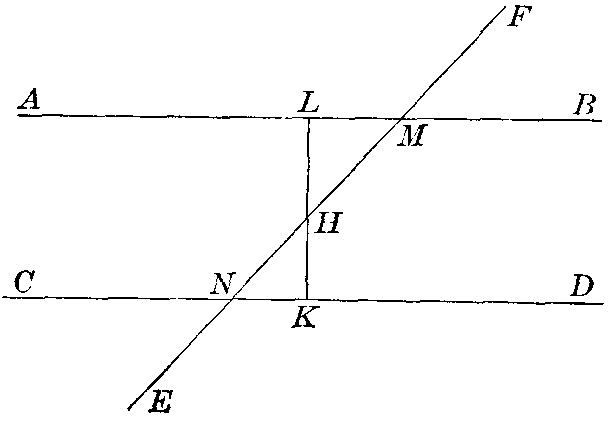
\includegraphics[width=50mm]{fig03.png}
\end{figure}

\item[10.~Theorem.] \emph{If two lines cut a third at the same angle,
that is, so that corresponding angles are equal, a line can be drawn
that is perpendicular to both.}

\textbf{Proof.} Let the angles $FMB$ and $MND$ be equal, and through
$H$, the middle point of $MN$, draw $LK$ perpendicular to $CD$; then
$LK$ will also be perpendicular to $AB$. For the two triangles $LMH$
and $KNH$ are equal by (3).

\item[11.~Theorem.] \emph{If two equal lines in a plane are erected
perpendicular to a given line, the line joining their extremities
makes equal angles with them and is bisected at right angles by a
third perpendicular erected midway between them.}

\newpage
\begin{figure}[h]
\centering
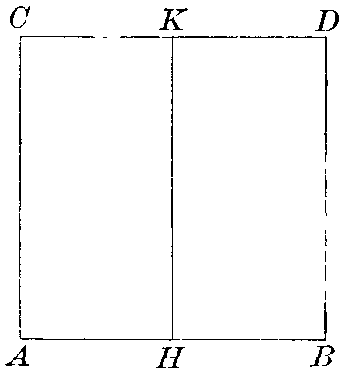
\includegraphics[width=40mm]{fig04.png}
\end{figure}

\textbf{Let} $AC$ and $BD$ be perpendicular to $AB$, and suppose
$AC$ and $BD$ equal. The angles at $C$ and $D$ made with a line
joining these two points are equal, and the perpendicular $HK$
erected at the middle point of $AB$ is perpendicular to $CD$ at its
middle point.

Proved by superposition.

\item[12.~Theorem.] \emph{Given as in the last proposition two
perpendiculars and a third perpendicular erected midway between
them; any line cutting this third perpendicular at right angles, if
it cuts the first two at all, will cut off equal lengths on them and
make equal angles with them.}

Proved by superposition.

\begin{figure}[h]
\centering
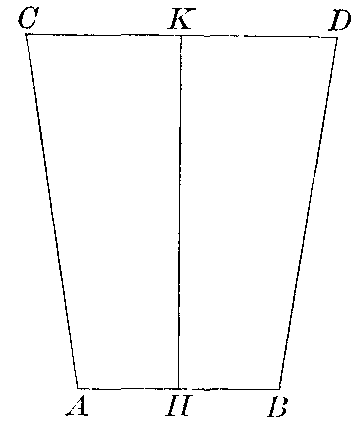
\includegraphics[width=40mm]{fig05.png}
\end{figure}

\textbf{Corollary.} \emph{The last two propositions hold true if the
angles at $A$ and $B$ are equal acute or equal obtuse angles, $HK$
being perpendicular to $AB$ at its middle point. If $AC = BD$, the
angles at $C$ and $D$ are equal, and $HK$ is perpendicular to $CD$
at its middle point: or, if $CD$ is perpendicular to $HK$ at any
point, $K$, and intersects $AC$ and $BD$, it it will cut off equal
distances on these two lines and make equal angles with them.}
\end{description}

\section{Propositions Which Are True for Restricted Figures}

The following propositions are true at least for figures whose lines
do not exceed a certain length. That is, if there is any exception,
it is in a case where we cannot apply the theorem or some step of
the proof on account of the length of some of the lines. For
convenience we shall use the word \emph{restricted} in this sense
and say that a theorem is true for restricted figures or in any
restricted portion of the plane.

\begin{figure}[h]
\centering
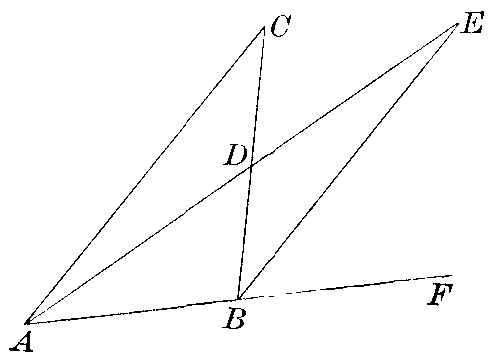
\includegraphics[width=40mm]{fig06.png}
\end{figure}

\begin{description}
\item[1.~Theorem.] \emph{The exterior angle of a triangle is
greater than either opposite interior angle} (Euclid, I, 16).

\textbf{Proof.} Draw $AD$ from $A$ to the middle point of the
opposite side and produce it to $E$, making $DE = AD$. The two
triangles $ADC$ and $EBD$ are equal, and the angle $FBD$, being
greater than the angle $EBD$, is greater than $C$.

\textbf{Corollary.} \emph{At least two angles of a triangle are
acute.}

\item[2.~Theorem.] \emph{If two angles of a triangle are equal, the
opposite sides are equal and the triangle is isosceles.}

\begin{figure}[h]
\centering
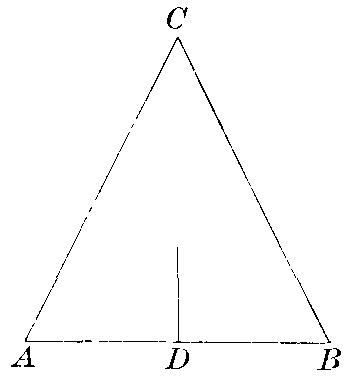
\includegraphics[width=40mm]{fig07.png}
\end{figure}

\textbf{Proof.} The perpendicular erected at the middle point of the
base divides the triangle into two figures which may be made
to coincide and are equal. This perpendicular, therefore,
passes through the vertex, and the two sides opposite the
equal angles of the triangle are equal.

\item[3.~Theorem.] \emph{In a triangle with unequal angles the
side opposite the greater of the angles is greater than the side
opposite the smaller; and conversely, if the sides of a triangle are
unequal the opposite angles are unequal, and the greater angle lies
opposite the greater side.}

\item[4.~Theorem.] \emph{If two triangles have two sides of one
equal, respectively, to two sides of the other, but the included
angle of the first greater than the included angle of the second,
the third side of the first is greater than the third side of the
second; and conversely, if two triangles have two sides of one
equal, respectively, to two sides of the other, but the third side
of the first greater than the third side of the second, the angle
opposite the third side of the first is greater than the angle
opposite the third side of the second.}

\item[5.~Theorem.] \emph{The sum of two lines drawn from any point
to the extremities of a straight line is greater than the sum of two
lines similarly drawn but included by them.}

\item[6.~Theorem.] \emph{Through any point one perpendicular only
can be drawn to a straight line.}

\begin{figure}[h]
\centering
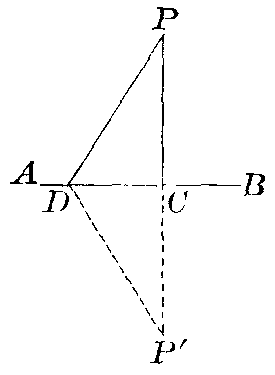
\includegraphics[width=30mm]{fig08.png}
\end{figure}

\textbf{Proof.} Let $P'$ be the position which $P$ would take if the
plane were revolved about $AB$ into coincidence with itself. If we
could have two perpendiculars, $PC$ and $PD$, from $P$ to $AB$, then
$CP'$ and $DP'$ would be continuations of these lines and we should
have two different straight lines joining $P$ and $P'$, which is
impossible.

\textbf{Corollary.} \emph{Two right triangles are equal when the
hypothenuse and an acute angle of one are equal, respectively, to
the hypothenuse and an acute angle of the other.}

\item[7.~Theorem.] \emph{The perpendicular is the shortest line that
can be drawn from a point to a straight line.}

\textbf{Corollary.} \emph{In a right triangle the hypothenuse is
greater than either of the two sides about the right angle.}

\item[8.~Theorem.] \emph{If oblique lines drawn from a point in a
perpendicular to a line cut off unequal distances from the foot of
the perpendicular, they are unequal, and the more remote is the
greater; and conversely, if two oblique lines drawn from a point in
a perpendicular are unequal, the greater cuts off a greater distance
from the foot of the perpendicular.}

\item[9.~Theorem.] \emph{If a perpendicular is erected at the middle
point of a straight line, any point not in the perpendicular is
nearer that extremity of the line which is on the same side of the
perpendicular.}

\textbf{Corollary.} \emph{Two points equidistant from the
extremities of a straight line determine a perpendicular to the line
at its middle point.}

\item[10.~Theorem.] \emph{Two triangles are equal when they have
three sides of one equal, respectively, to three sides of the
other.}

\item[11.~Theorem.] \emph{If two lines in a plane erected
perpendicular to a third are unequal, the line joining their
extremities makes unequal angles with them, the greater angle with
the shorter perpendicular.}

\begin{figure}[h]
\centering
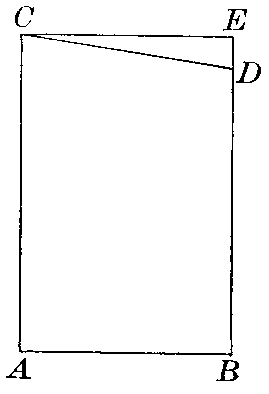
\includegraphics[width=25mm]{fig09.png}
\end{figure}

\textbf{Proof.} Suppose $AC > BD$. Produce $BD$, making $BE = AC$.
Then $BEC = ACE$. But $BDC > BEC$, by (1), and $ACD$ is a part of
$ACE$. Therefore, all the more $BDC > ACD$.

\item[12.~Theorem.] \emph{If the two angles at $C$ and $D$ are equal,
the perpendiculars are equal, and if the angles are unequal, the
perpendiculars are unequal, and the longer perpendicular makes the
smaller angle.}

\newpage
\item[13.~Theorem.] \emph{If two lines are perpendicular to a third,
points on either equidistant from the third are equidistant from the
other.}

\begin{figure}[h]
\centering
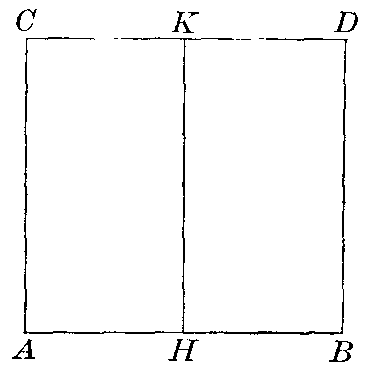
\includegraphics[width=30mm]{fig10.png}
\end{figure}

\textbf{Proof.} Let $AB$ and $CD$ be perpendicular to $HK$, and on
$CD$ take any two points, $C$ and $D$, equidistant from $K$; then
$C$ and $D$ will be equidistant from $AB$. For by superposition we
can make $D$ fall on $C$, and then $DB$ will coincide with $CA$ by
(6).
\end{description}

\medskip The following propositions of Solid Geometry depend directly
on the preceding and hold true at least for any restricted portion
of space.

\begin{description}
\item[14.~Theorem.] \emph{If a line is perpendicular to two
intersecting lines at their intersection, it is perpendicular to all
lines of their plane passing through this point.}

\item[15.~Theorem.] \emph{If two planes are perpendicular, a line
drawn in one perpendicular to their intersection is perpendicular to
the other, and a line drawn through any point of one perpendicular
to the other lies entirely in the first.}

\item[16.~Theorem.] \emph{If a line is perpendicular to a plane,
any plane through that line is perpendicular to the plane.}

\item[17.~Theorem.] \emph{If a plane is perpendicular to each of
two intersecting planes, it is perpendicular to their intersection.}
\end{description}

\section{The Three Hypotheses}

The angles at the extremities of two equal perpendiculars are either
right angles, acute angles, or obtuse angles, at least for
restricted figures. We shall distinguish the three cases by speaking
of them as the hypothesis of the right angle, the hypothesis of the
acute angle, and the hypothesis of the obtuse angle, respectively.

\begin{description}
\item[1.~Theorem.] \emph{The line joining the extremities of two
equal perpendiculars is, at least for any restricted portion of the
plane, equal to, greater than, or less than the line joining their
feet in the three hypotheses, respectively.}

\newpage
\begin{figure}[h]
\centering
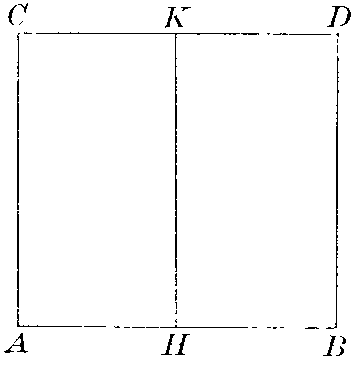
\includegraphics[width=35mm]{fig11.png}
\end{figure}

\textbf{Proof.} Let $AC$ and $BD$ be the two equal perpendiculars
and $HK$ a third perpendicular erected at the middle point of $AB$.
Then $HA$ and $KC$ are perpendicular to $HK$, and $KC$ is equal to,
greater than, or less than $HA$, according as the angle at $C$ is
equal to, less than, or greater than the angle at $A$ (II, 12).
Hence, $CD$, the double of $KC$, is equal to, greater than, or less
than $AB$ in the three hypotheses, respectively.

\textbf{Conversely,} if $CD$ is given equal to, greater than, or
less than $AB$, there is established for this figure the first,
second, or third hypothesis, respectively.

\textbf{Corollary.} \emph{If a quadrilateral has three right angles,
the sides adjacent to the fourth angle are equal to, greater than,
or less than the sides opposite them, according as the fourth angle
is right, acute, or obtuse.}

\item[2.~Theorem.] \emph{If the hypothesis of a right angle is true
in a single case in any restricted portion of the plane, it holds
true in every case and throughout the entire plane.}

\begin{figure}[h]
\centering
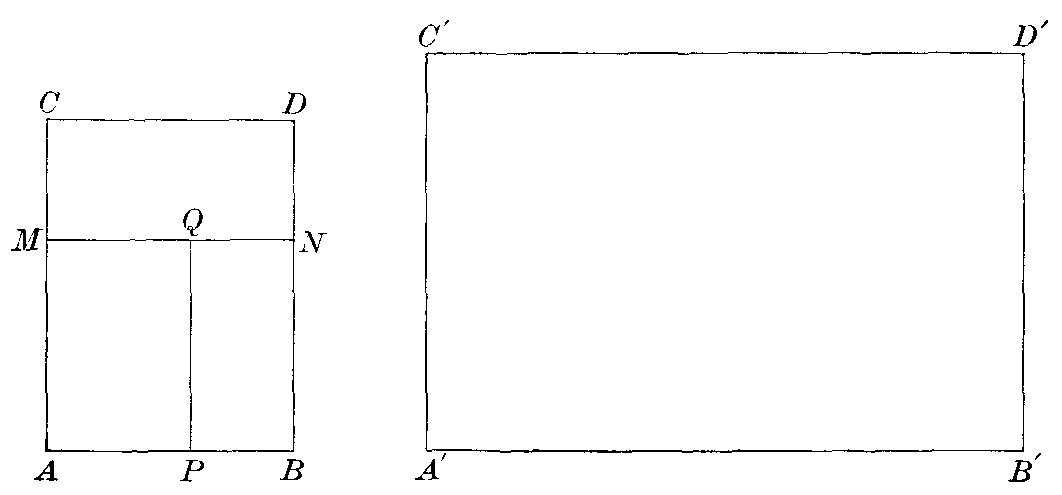
\includegraphics[width=75mm]{fig12.png}
\end{figure}

\textbf{Proof.} We have now a rectangle; that is, a quadrilateral
with four right angles. By the corollary to the last proposition,
its opposite sides are equal. Equal rectangles can be placed
together so as to form a rectangle whose sides shall be any given
multiples of the corresponding sides of the given rectangle.

Now let $A'B'$ be any given line and $A'C'$ and $B'D'$ two equal
lines perpendicular to $A'B'$ at its extremities. Divide $A'C'$, if
necessary, into a number of equal parts so that one of these parts
shall be less than $AC$, and on $AC$ and $BD$ lay off $AM$ and $BN$
equal to one of these parts, and draw $MN$. $ABNM$ is a rectangle;
for otherwise $MN$ would be greater than or less than $AB$ and $CD$,
and the angles at $M$ and $N$ would all be acute angles or all
obtuse angles, which is impossible, since their sum is exactly four
right angles. Again, divide $A'B'$ into a sufficient number of equal
parts, lay off one of these parts on $AB$ and on $MN$, and form the
rectangle $APQM$. Rectangles equal to this can be placed together so
as exactly to cover the figure $A'B'D'C'$, which must therefore
itself be a rectangle.

\item[3.~Theorem.] \emph{If the hypothesis of the acute angle or the
hypothesis of the obtuse angle holds true in a single case within a
restricted portion of the plane, the same hypothesis holds true for
every case within any such portion of the plane.}

\begin{figure}[h]
\centering
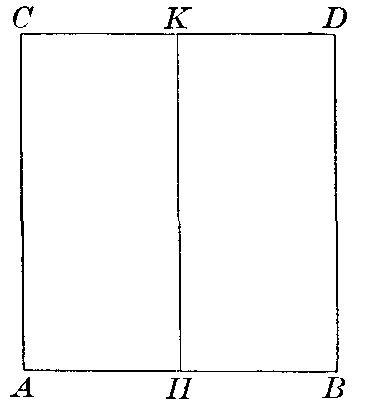
\includegraphics[width=35mm]{fig13.png}
\end{figure}

\textbf{Proof.} Let $CD$ move along $AC$ and $BD$, always cutting
off equal distances on these two lines; or, again, let $AC$ and $BD$
move along on the line $AB$ towards $HK$ or away from $HK$, always
remaining perpendicular to $AB$ and their feet always at equal
distances from $H$. The angles at $C$ and $D$ vary continuously and
must therefore remain acute or obtuse, as the case may be, or at
some point become right angles. There would then be established the
hypothesis of the right angle, and the hypothesis of the acute angle
or of the obtuse angle could not exist even in the single case
supposed.

The angles at $C$ and $D$ could not become zero nor $180^\circ$ in a
restricted portion of the plane; for then the three lines $AC$,
$CD$, and $BD$ would be one and the same straight line.

\item[4.~Theorem.] \emph{The sum of the angles of a triangle, at
least in any restricted portion of the plane, is equal to, less
than, or greater than two right angles, in the three hypotheses,
respectively.}

\newpage
\begin{figure}[h]
\centering
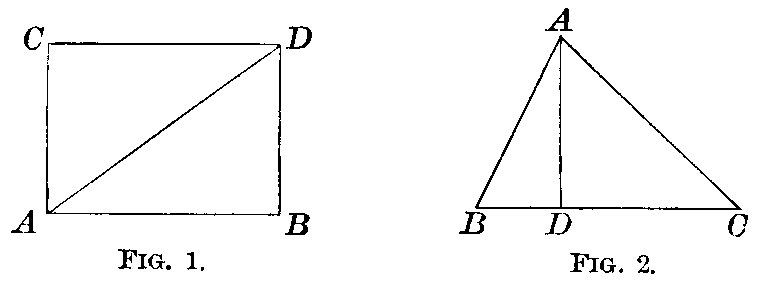
\includegraphics[width=80mm]{fig14.png}
\end{figure}

\textbf{Proof.} Given any triangle, $ABD$ (Fig.~1), with right angle
at $B$, draw $AC$ perpendicular to $AB$ and equal to $BD$. In the
triangles $ADC$ and $DAB$, $AC=BD$ and $AD$ is common, but $DC$ is
equal to, greater than, or less than $AB$ in the three hypotheses,
respectively. Therefore, $DAC$ is equal to, greater than, or less
than $ADB$ in the three hypotheses, respectively (II, 4). Adding
$BAD$ to both of these angles, we have $ADB + BAD$ equal to, or
greater than the right angle $BAC$.

Now at least two angles of any restricted triangle are acute. The
perpendicular, therefore, from the vertex of the third angle upon
its opposite side will meet this side within the triangle and divide
the triangle into two right triangles. Therefore, in any restricted
triangle the sum of the angles is equal to, less than, or greater
than two right angles in the three hypotheses, respectively.

We will call the amount by which the angle-sum of a triangle exceeds
two right angles its excess. The excess of a polygon of $n$ sides is
the amount by which the sum of its angles exceeds $n-2$ times two
right angles.

It will not change the excess if we count as additional vertices any
number of points on the sides, adding to the sum of the angles two
right angles for each of these points.

\item[5.~Theorem.] \emph{The excess of a polygon is equal to the
sum of the excesses of any system of triangles into which it may be
divided.}

\begin{figure}[h]
\centering
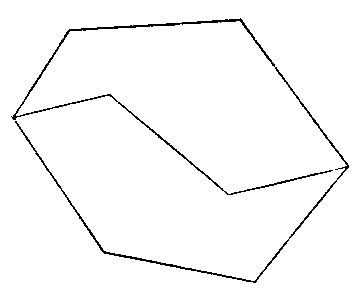
\includegraphics[width=30mm]{fig15.png}
\end{figure}

\textbf{Proof.} If we divide a polygon into two polygons by a
straight or broken line, we may assume that the two points where it
meets the boundary are vertices. If the dividing line is a broken
line, broken at $p$ points, an the sides of the two polygons will be
the sides of the original polygon, together with the $p+1$ parts
into which the dividing line is separated by the $p$ points, each
part counted twice.

\textbf{Let} $S$ be the sum of the angles of the original polygon,
and $n$ the number of its sides. Let $S'$ and $n'$, $S''$ and $n''$
have the same meanings for the two polygons into which it is
divided. Then we have, writing $R$ for the right angle,
\begin{align*}
S' + S'' &= S + 4pR, \\
\intertext{and}
n' + n'' &= n + 2(p+1). \\
\intertext{Therefore,}
S' - 2(n'-2)R + S'' - 2(n''-2)R &= S + 4pR - 2(n+2p-2)R \\
&= S-2(n-2)R.
\end{align*}

Any system of triangles into which a polygon may be divided is
produced by a sufficient number of repetitions of the above process.
Always the excess of the polygon is equal to the sum of the excesses
of the parts into which it is divided.

We may extend the notion of excess and apply it to any combination
of different portions of the plane hounded completely by straight
lines.

Instead of considering the sum of the angles of a polygon, we may
take the sum of the exterior angles. The amount by which this sum
falls short of four right angles equals the excess of the polygon.
We may speak of it as the deficiency of the exterior angles.

\begin{figure}[h]
\centering
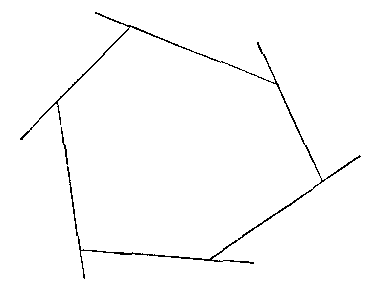
\includegraphics[width=30mm]{fig16.png}
\end{figure}

The sum of the exterior angles is the amount by which we turn in
going completely around the figure, turning at each vertex from one
side to the next. If we are considering a combination of two or more
polygons, we must traverse the entire boundary and so as always to
have the area considered on one side, say on the left.

\item[6.~Theorem.] \emph{The excess of polygons is always zero,
always negative, or always positive.}

\textbf{Proof.} We know that this theorem is true of restricted
triangles, but any finite polygon may be divided into a finite
number of such triangles, and by the last theorem the excess of the
polygon is equal to the sum of the excesses of the triangles.

When the excess is negative, we may call it deficiency, or speak of
the excess of the exterior angles.

\textbf{Corollary.} \emph{The excess of a polygon is numerically
greater than the excess of any part which may be cut off from it by
straight lines, except in the first hypothesis, when it is zero.}
\end{description}

\medskip The following theorems apply to the second and third
hypotheses.

\begin{description}
\item[7.~Theorem.] \emph{By diminishing the sides of a triangle,
or even one side while the other two remain less than some fixed
length, we can diminish its area indefinitely, and the sum of its
angles will approach two right angles as limit.}

\begin{figure}[h]
\centering
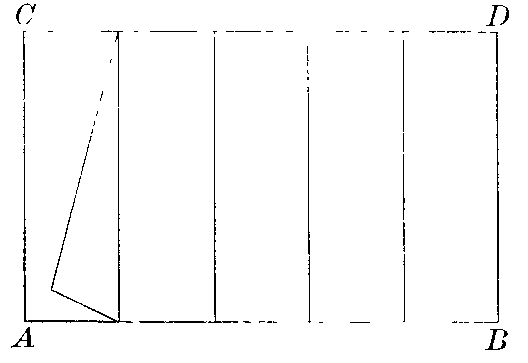
\includegraphics[width=50mm]{fig17.png}
\end{figure}

\textbf{Proof.} Let $ABDC$ be a quadrilateral with three right
angles, $A$, $B$, and $C$. A perpendicular moving along $AB$ will
constantly increase or decrease; for if it could increase a part of
the way and decrease a part of the way there would be different
positions where the perpendiculars have the same length; a
perpendicular midway between them would be perpendicular to $CD$
also, and we should have a rectangle.

Divide $AB$ into $n$ equal parts, and draw perpendiculars through
the points of division. The quadrilateral is divided into $n$
smaller quadrilaterals, which can be applied one to another, having
a side and two adjacent right angles the same in all. Beginning at
the end where the perpendicular is the shortest, each quadrilateral
can be placed entirely within the next. Therefore, the first has its
area less than $\nicefrac{1}{n}$th of the area of the original
quadrilateral, and its deficiency or excess less than
$\nicefrac{1}{n}$th of the deficiency or excess of the whole. Now
any triangle whose sides are all less than $AC$ or $BD$, and one of
whose sides is less than one of the subdivisions of $AB$, can be
placed entirely within this smallest quadrilateral. Such a triangle
has its area and its deficiency or excess less than
$\nicefrac{1}{n}$th of the area and of the deficiency or excess of
the original quadrilateral.

Thus, a triangle has its area and deficiency or excess less than any
assigned area and deficiency or excess, however small, if at least
one side is taken sufficiently small, the other two sides not being
indefinitely large.

\newpage
\item[8.~Theorem.] \emph{Two triangles having the same deficiency or
excess have the same area.}

\begin{figure}[h]
\centering
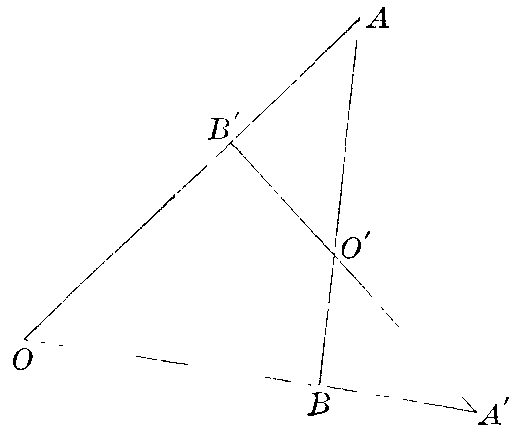
\includegraphics[width=40mm]{fig18.png}
\end{figure}

\textbf{Proof.} Let $AOB$ and $A'OB'$ have the same deficiency or
excess and an angle of one equal to an angle of the other. If we
place them together so that the equal angles coincide, the triangles
will coincide and be entirely equal, or there will be a
quadrilateral common to the two, and, besides this, two smaller
triangles having an angle the same in both and the same deficiency
or excess. Putting these together, we find again a quadrilateral
common to both and a third pair of triangles having an angle the
same in both and the same deficiency or excess. We may continue this
process indefinitely, unless we come to a pair of triangles which
coincide; for at no time can one triangle of a pair be contained
entirely within the other, since they have the same deficiency or
excess.

Let $so$ denote the sum of the sides opposite the equal angles of
the first two triangles, $sa$ the sum of the adjacent sides, and
$s'a$ that portion of the adjacent sides counted twice, which is
common to the two triangles when they are placed together. Writing
$o'$ and $a'$ for the second pair of triangles, $o''$ and $a'$ for
the third pair, etc., we have
\begin{gather*}
\begin{aligned}
sa   &= s'a + so',                 & so   &= sa',  \\
sa'  &= s'a' + so'',               & so'  &= sa'', \\
sa'' &= s'a'' + so'''\text{, etc.} & so'' &= sa''' \text{, etc.}
\end{aligned}\\
\begin{aligned}
\therefore sa  &= s'a  + s'a''  + s'a^{IV} + \ldots, \\
           sa' &= s'a' + s'a''' + s'a^{V}  + \ldots.
\end{aligned}
\end{gather*}

Therefore, the expressions $s'a$, $s'a'$, $s'a''$, $\cdots$ diminish
indefinitely. Each of these is made up of a side counted twice from
one and a side counted twice from the other of a pair of triangles.
Thus, if we carry the process sufficiently far, the remaining
triangles can be made to have at least one side as small as we
please, while all the sides diminish and are less, for example, than
the longest of the sides of the original triangles. Therefore, the
areas of the remaining triangles diminish indefinitely, and as the
difference of the areas remains the same for each pair of triangles,
this difference must be zero. The triangles of each pair and, in
particular, the first two triangles have the same area.

\begin{figure}[ht]
\centering
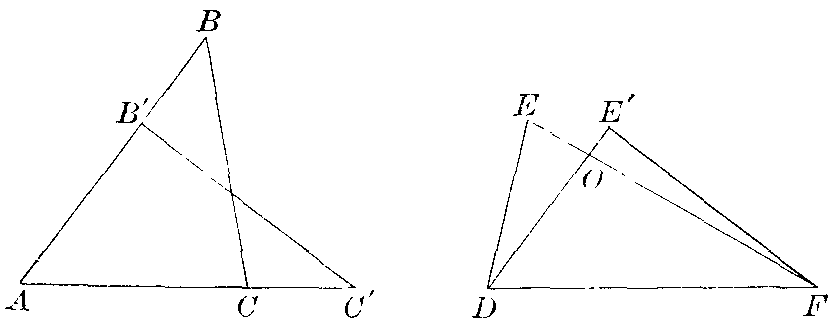
\includegraphics[width=70mm]{fig19.png}
\end{figure}

Let $ABC$ and $DEF$ have the same deficiency or excess, and suppose
$AC<DF$.  Produce $AC$ to $C'$, making $AC'$ = $DF$. Then there is
some point, $B'$, on $AB$ between $A$ and $B$ such that $AB'C'$ has
the same deficiency or excess and the same area as $ABC$. Place
$AB'C'$ upon $DEF$ so that AC' will coincide with $DF$, and let
$DE'F$ be the position which it takes. If the triangles do not
coincide, the vertex of each opposite the common side $DF$ lies
outside of the other. The two triangles have in common a triangle,
say $DOF$, and besides this there remain of the two triangles two
smaller triangles which have one angle the same in both and the same
deficiency or excess. These two triangles, and therefore the
original triangles, have the same area.

\item[9.~Theorem.] \emph{The areas of any two triangles are
proportional to their deficiencies or excesses.}

\begin{figure}[h]
\centering
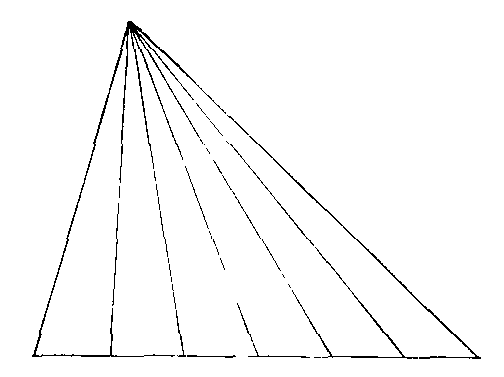
\includegraphics[width=40mm]{fig20.png}
\end{figure}

\textbf{Proof.} A triangle may be divided into $n$ smaller triangles
having equal deficiencies or excesses and equal areas by lines drawn
from one vertex to points of the opposite side. Each of these
triangles has for its deficiency or excess $\nicefrac{1}{n}$th of
the deficiency or excess of the original triangle, and for its area
$\nicefrac{1}{n}$th of the area of the original triangle.

When the deficiencies or excesses of two triangles are
commensurable, say in the ratio $m: n$, we can divide them into $m$
and $n$ smaller triangles, respectively, all having the same
deficiency or excess and the same area. The areas of the given
triangles will therefore be in the same ratio, $m : n$.

\newpage
\begin{figure}[h]
\centering
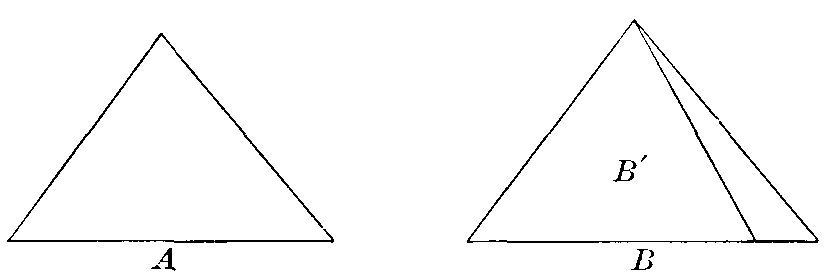
\includegraphics[width=70mm]{fig21.png}
\end{figure}

When the deficiencies or excesses of two triangles, $A$ and $B$, are
not commensurable, we may divide one triangle, $A$, as above, into
any number of equivalent parts, and take parts equivalent to one of
these as many times as possible from the other, leaving a remainder
which has a deficiency or excess less than the deficiency or excess
of one of these parts. The portion taken from the second triangle
forms a triangle, $B'$. $A$ and $B'$ have their areas proportional
to their deficiencies or excesses, these being commensurable. Now
increase indefinitely the number of parts into which $A$ is divided.
These parts will diminish indefinitely, and the remainder when we
take $B'$ from $B$ will diminish indefinitely. The deficiency or
excess and the area of $B'$ will approach those of $B$, and the
triangles $A$ and $B$ have their areas and their deficiencies or
excesses proportional.

\textbf{Corollary.} \emph{The areas of two polygons are to each
other as their deficiencies or excesses.}

\item[10.~Theorem.] \emph{Given a right triangle with a fixed angle;
if the sides of the triangle diminish indefinitely, the ratio of the
opposite side to the hypothenuse and the ratio of the adjacent side
to the hypothenuse approach as limits the sine and cosine of this
angle.}

\textbf{Proof.} Lay off on the hypothenuse any number of equal
lengths. Through the points of division $A_1$, $A_2$, $\cdots$ draw
perpendiculars $A_1C_1$, $A_2C_2$, $\cdots$ to the base, and to
these lines produced draw perpendiculars $A_2D_1$, $A_3D_2$,
$\cdots$ each from the next point of division of the hypothenuse.

\P~The triangles $OA_1C_1$ and $A_2A_1D_1$ are equal (II, 6, Cor.).
\begin{align*}
  C_2A_2 &\gtrless C_1D_1 &&\text{and} & C_1C_2 &\lessgtr D_1A_2;\\
  \intertext{therefore,}
  \frac{C_2A_2}{OA_2} &\gtrless \frac{C_1A_1}{OA_1}
  &&\text{and} & \frac{OC_2}{OA_2} &\lessgtr \frac{OC_1}{OA_1},
\end{align*}
the upper sign being for the second hypothesis and the lower
sign for the third hypothesis.

\newpage
\begin{figure}[h]
\centering
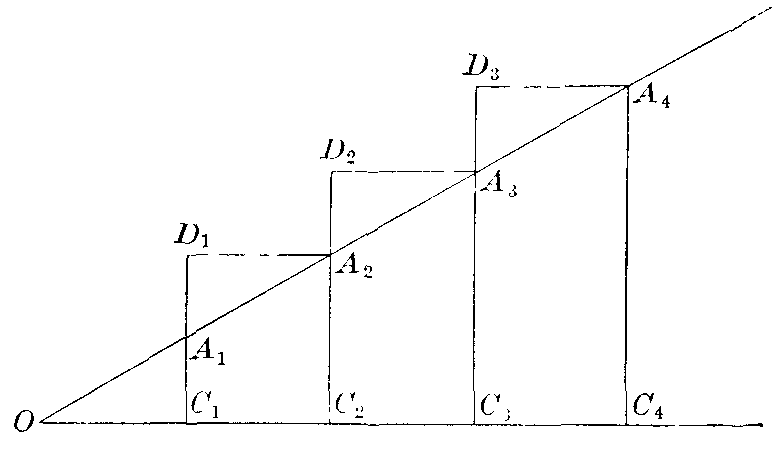
\includegraphics[width=70mm]{fig22.png}
\end{figure}

\P~Assume
\begin{equation*}
  \frac{C_{r-1}A_{r-1}}{OA_{r-1}}
  \gtrless \frac{C_{r-2}A_{r-2}}{OA_{r-2}}
  \gtrless \dots
  \gtrless \frac{C_1A_1}{OA_1},
\end{equation*}
and
\begin{equation*}
  \frac{OC_{r-1}}{OA_{r-1}}
  \lessgtr \frac{OC_{r-2}}{OA_{r-2}}
  \lessgtr \dots
  \lessgtr \frac{OC_1}{OA_1}.
\end{equation*}

\P~Since
\begin{align*}
  OA_{r-1} &= (r-1) OA_1,\\
\intertext{and also}
           &= (r-1) A_{r-1}A_r,
\end{align*}
the inequalities
\begin{equation*}
  \frac{OC_1}{OA_1} \gtrless \frac{OC_{r-1}}{OA_{r-1}} \quad
  \text{and}\quad
  \frac{C_1A_1}{OA_1} \lessgtr \frac{C_{r-1}A_{r-1}}{OA_{r-1}}
\end{equation*}
applied to the angle at $A_{r-1}$ become
\begin{equation*}
  \frac{A_{r-1}D_{r-1}}{A_{r-1}A_r} \gtrless
  \frac{C_{r-1}A_{r-1}}{OA_{r-1}}\quad
  \text{and}\quad
  \frac{D_{r-1}A_r}{A_{r-1}A_r} \lessgtr
  \frac{OC_{r-1}}{OA_{r-1}}.
\end{equation*}

\P~The first of these two inequalities may be written
\begin{equation*}
  \frac{A_{r-1}D_{r-1}}{C_{r-1}A_{r-1}} \gtrless
  \frac{A_{r-1}A_r}{OA_{r-1}}.
\end{equation*}

\P~Add 1 to both members,
\begin{align*}
\frac{C_{r-1}D_{r-1}}{C_{r-1}A_{r-1}} &\gtrless
                                            \frac{OA_r}{OA_{r-1}}, \\
\intertext{or}
\frac{C_{r-1}D_{r-1}}{OA_r} &\gtrless
                                   \frac{C_{r-1}A{r-1}}{OA_{r-1}}, \\
\intertext{But}
C_rA_r &\gtrless C_{r-1}D_{r-1}, \\
\intertext{therefore}
\frac{C_rA_r}{OA_r} &\gtrless \frac{C_{r-1}A_{r-1}}{OA_{r-1}}, \\
\end{align*}

\P~Again,
\begin{align*}
C_{r-1}C_r &\lessgtr D_{r-1}A_r. \\
\intertext{Hence, from the second inequality above, we have}
\frac{C_{r-1}C_r}{A_{r-1}A_r} &\lessgtr \frac{OC_{r-1}}{OA_{r-1}}, \\
\intertext{or}
\frac{C_{r-1}C_r}{OC_{r-1}} &\lessgtr \frac{A_{r-1}A_r}{OA_{r-1}}. \\
\end{align*}

\P~Add 1 to both members,
\begin{align*}
\frac{OC_r}{OC_{r-1}} &\lessgtr \frac{OA_r}{OA_{r-1}}, \\
\intertext{or}
\frac{OC_r}{OA_r} &\lessgtr \frac{OC_{r-1}}{OA_{r-1}}
\end{align*}

The ratios $\dfrac{CA}{OA}$ and $\dfrac{OC}{OA}$ being less than 1,
and always increasing or always decreasing when the hypothenuse
decreases, approach definite limits. These limits are continuous
functions of $A$; if we vary the angle of any right triangle
continuously, keeping the hypothenuse some fixed length, the other
two sides will vary continuously, and the limits of their ratios to
the hypothenuse must, therefore, vary continuously.

Calling the limits for the moment $sA$ and $cA$, we may extend their
definition, as in Trigonometry, to any angles, and prove that all
the formulæ of the sine and cosine hold for these functions. Then
for certain angles, $30^\circ$, $45^\circ$, $60^\circ$, we can prove
that they have the same values as the sine and cosine, and their
values for all other angles as determined from their values for
these angles will be the same as the corresponding values of the
sine and cosine.

\begin{figure}[ht]
\centering
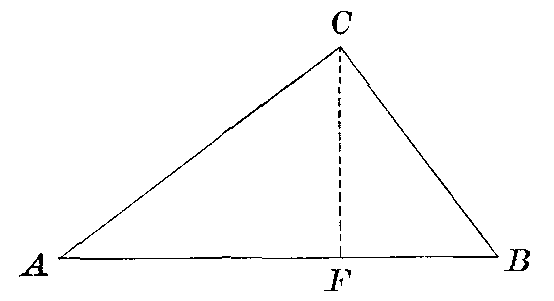
\includegraphics[width=50mm]{fig23.png}
\end{figure}

Draw a perpendicular, $CF$, from the right angle $C$ to the
hypothenuse $AB$. The angle $FCB$ is not equal to $A$, but the
difference, being proportional to the difference of areas of the two
triangles $ABC$ and $FBC$, diminishes indefinitely when the sides of
the triangles diminish. From the relation
\begin{equation*}
\frac{AF}{AC}\cdot\frac{AC}{AB} +
    \frac{FB}{BC}\cdot\frac{BC}{AB} = 1,
\end{equation*}
we have, by passing to the limit,
\begin{equation*}
(cA)^2 + (sA)^2 = 1.
\end{equation*}

Let $x$ and $y$ be any two acute angles, and draw the figures used
to prove the formulas for the sine and cosine of the sum of two
angles.

The angles $x$ and $y$ remaining fixed, we can imagine all of the
lines to decrease indefinitely, and the functions $sx$, $ex$, $sy$,
etc., are the limits of certain ratios of these lines.
\begin{gather*}
\begin{aligned}
\frac{CA}{OA} &= \frac{CE}{OB}\cdot\frac{OB}{OA}
                                + \frac{EA}{BA}\cdot\frac{BA}{OA}, \\
\pm \frac{CA}{OA} &= \frac{OD}{OB}\cdot\frac{OB}{OA}
                                - \frac{CD}{BA}\cdot\frac{BA}{OA}, \\
\end{aligned} \\
\left(-\frac{OC}{OA} \text{ in the second figure} \right).
\end{gather*}

The angles at $M$ are equal in the two triangles $EMB$ and $CMO$,
and we may write
\begin{equation*}
\frac{CM}{OM} = \frac{ME + \delta}{MB}
                              = \frac{ME \pm CM + \delta}{MB \pm OM},
\end{equation*}
where $\delta$ has the limit zero.
\begin{equation*}
\therefore \lim \frac{CE}{OB} = \lim\frac{CM}{OM} = sx.
\end{equation*}

\newpage
\begin{figure}[h]
\centering
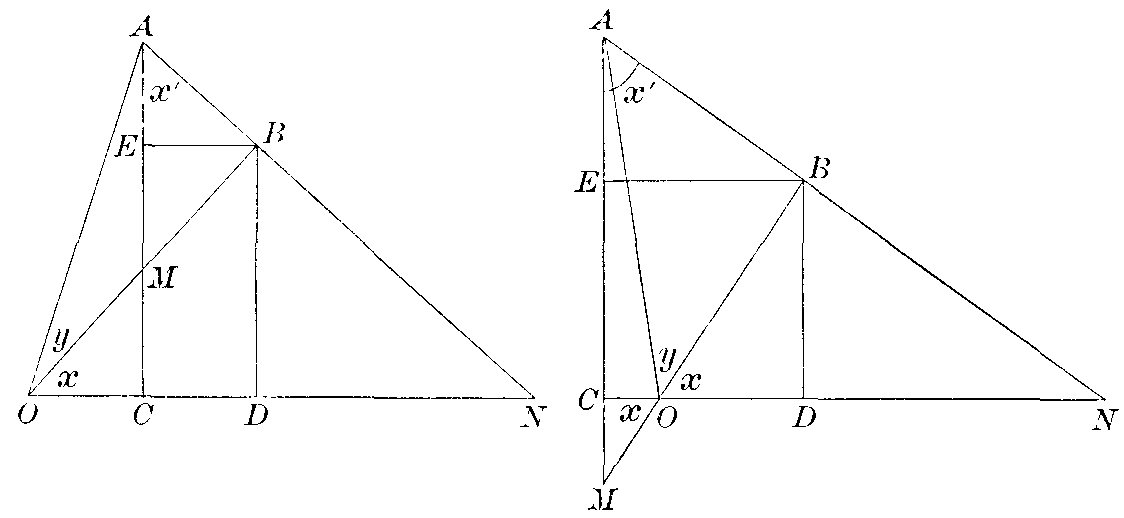
\includegraphics[width=80mm]{fig24.png}
\end{figure}

The angle $EAB$, or $x'$, is not the same as $x$, but differs from
$x$ only by an amount which is proportional to the difference of the
areas of the triangles $OMC$ and $MAB$, and which, therefore,
diminishes indefinitely. Thus, the limits of $sx'$ and $cx'$ are
$sx$ and $cx$.

Finally, as the two triangles $ACN$ and $BDN$ have the angle $N$ in
common, we may write
\begin{equation*}
\frac{DN}{BN} = \frac{CN + \delta '}{AN}
                                = \frac{CN - DN + \delta '}{AN - BN},
\end{equation*}
where the limit of $\delta'$ is zero.
\begin{equation*}
\therefore \lim \frac{CD}{AB} = \lim\frac{CN}{AN} = sx.
\end{equation*}

Now at the limits our identities become
\begin{align*}
s(x+y) &=  sx \cdot cy + cx \cdot sy, \\
c(x+y) &=  cx \cdot cy - sx \cdot sy.
\end{align*}

By induction, these formulæ are proved true for any angles. Other
formulæ sufficient for calculating the values of these functions
from their values for $30^\circ$, $45^\circ$, and $60^\circ$ are
obtained from these two by algebraic processes.

If the sides of an isosceles right triangle diminish indefinitely,
the angle does not remain fixed but approaches $45^\circ$, and the
ratios of the two sides to the hypothenuse approach as limits $s\
45^\circ$ and $c\ 45^\circ$. Therefore, these latter are equal, and
since the sum of their squares is 1, the value of each is
$\nicefrac{1}{\sqrt{2}}$, the same as the value of the sine and
cosine of $45^\circ$.

Again, bisect an equilateral triangle and form a triangle in which
the hypothenuse is twice one of the sides. When the sides diminish,
preserving this relation, the angles approach $30^\circ$ and
$60^\circ$. Therefore, the functions, $s$ and $c$, of these angles
have values which are the same as the corresponding values of the
sine and cosine of the same angles.

\textbf{Corollary.} \emph{When any plane triangle diminishes
indefinitely, the relations of the sides and angles approach those
of the sides and angles of plane triangles in the ordinary geometry
and trigonometry with which we are familiar.}

\item[11.~Theorem.] \emph{Spherical geometry is the same in the
three hypotheses, and the formula of spherical trigonometry are
exactly those of the ordinary spherical trigonometry.}

\textbf{Proof.} On a sphere, arcs of great circles are proportional to
the angles which they subtend at the centre, and angles on a
sphere are the same as the diedral angles formed by the planes
of the great circles which are the sides of the angles. Their
relations are established by drawing certain plane triangles
which may be made as small as we please, and therefore may
be assumed to be like the plane triangles in the hypothesis
of a right angle. These relations are, therefore, those of the
ordinary Spherical Trigonometry.
\end{description}

\medskip The three hypotheses give rise to three systems of Geometry,
which are called the Parabolic, the Hyperbolic, and the Elliptic
Geometries. They are also called the Geometries of Euclid, of
Lobachevsky, and of Riemann. The following considerations exhibit
some of their chief characteristics.

\begin{figure}[h]
\centering
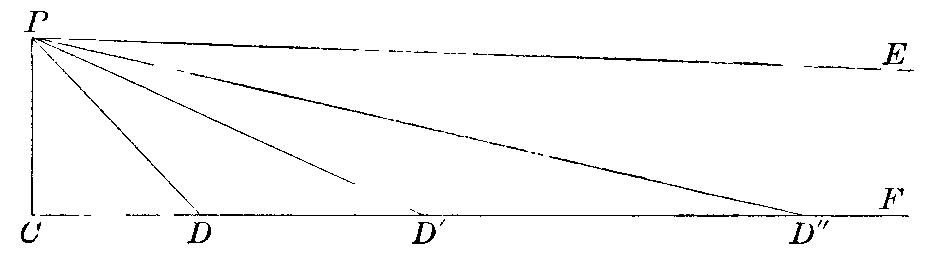
\includegraphics[width=80mm]{fig25.png}
\end{figure}

Given $PC$ perpendicular to a line, $CF$; on the latter we take
\begin{align*}
  CD    &= PC, \\
  DD'   &= PD, \\
  D'D'' &= PD',\ \text{etc.}
\end{align*}

\label{p27xref}Now if $PC$ is sufficiently short (restricted), it is
shorter than \emph{any} other line from $P$ to the line $CF$; for
any line as short as $PC$ or shorter would be included in a
restricted portion of the plane about the point $P$, for which the
perpendicular is the shortest distance from the point to the line.

Therefore,
\begin{align*}
  PD  &> PC,               &\therefore CD' &> 2CD,\\
  PD' &> PC,\ \text{etc.;} &          CD'' &> 3CD,\ \text{etc.}
\end{align*}

Again, in the three hypotheses, respectively,
\begin{align*}
  CPD    &\stackrel{=}{\lessgtr} \frac{\pi}{4}, &&\text{and}&
                         CDP &\stackrel{=}{\lessgtr} \frac{\pi}{4},\\
  DPD'   &\stackrel{=}{\lessgtr} \tfrac{1}{2} CPD, &&&
                    CD'P  &\stackrel{=}{\lessgtr} \tfrac{1}{2} CDP,\\
  D'PD'' &\stackrel{=}{\lessgtr} \tfrac{1}{2} DPD',\ \text{etc.,} &&&
        CD''P &\stackrel{=}{\lessgtr} \tfrac{1}{2} CD'P,\ \text{etc.}
\end{align*}

At $P$ we have a series of angles. In the first hypothesis there is
an infinite number of these angles, and the series forms a
geometrical progression of ratio $\nicefrac{1}{2}$, whose value is
exactly $\nicefrac{\pi}{2}$. In the second hypothesis there is also
an infinite number of these angles, and the terms of the series are
less than the terms of the geometrical progression. The value of the
series is, therefore, less than $\nicefrac{\pi}{2}$. In the third
hypothesis we have a series whose terms are greater than those of
the geometrical progression, and, therefore, whether the series is
convergent or divergent, we can get more than $\nicefrac{\pi}{2}$ by
taking a sufficient number of terms. In other words, we can get a
right angle or more than a right angle at $P$ by repeating this
process a certain finite number of times.

The angles at $D$, $D'$, $D''$, $\cdots$ are exactly equal to the
terms of the series of angles at $P$. In the first two hypotheses
they approach zero as a limit.

The distances $CD$, $CD'$, $CD''$, $\cdots$ increase each time by
more than a definite quantity, $CD$; therefore, if we repeat the
process an unlimited number of times, these distances will increase
beyond all limit. Thus, in the first and second hypotheses we prove
that a straight line must be of infinite length.

In the hypothesis of the obtuse angle the line perpendicular to $PC$
at the point $P$ will intersect $CF$ in a point at a certain finite
distance from $C$, one of the $D$'s, or some point between. On the
other side of $PC$ this same perpendicular will intersect $FC$
produced at the same distance. But we have assumed that two
different straight lines cannot intersect in two points; therefore,
for us the third hypothesis cannot be true unless the straight line
is of finite length returning into itself, and these two points are
one and the same point, its distance from $C$ in either direction
being one-half the entire length of the line. In this way, however,
we can build up a consistent Geometry on the third hypothesis, and
this Geometry it is which is called the Elliptic Geometry.

The constructions would have been the same, and very nearly all the
statements would have been the same, if we had taken $CD$ any
arbitrary length on $CF$.

The restriction which we have placed upon some of the propositions
of this chapter is necessary in the third hypothesis.

\newpage
\begin{figure}[h]
\centering
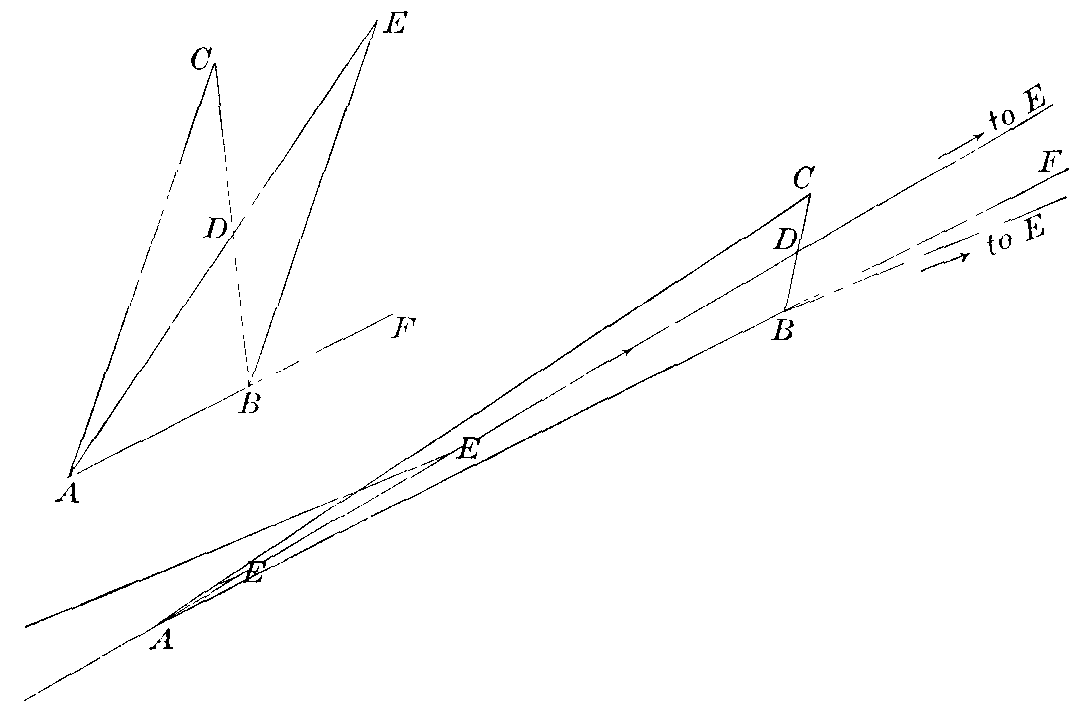
\includegraphics[width=80mm]{fig26.png}
\end{figure}

Thus, in the proof that the exterior angle of a triangle is greater
than the opposite interior angle, the line $AD$ drawn through the
vertex $A$ to the middle point $D$ of the opposite side was produced
so as to make $AE=2AD$. If $AD$ were greater than half the entire
length of the straight line determined by $A$ and $D$, this would
bring the point $E$ past the point $A$, and the angle $CBE$, which
is equal to the angle $C$, instead of being a part of the exterior
angle $CBF$, becomes greater than this exterior angle.

\begin{figure}[h]
\centering
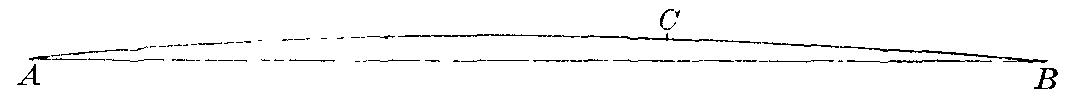
\includegraphics[width=80mm]{fig27.png}
\end{figure}

Again, if two angles of a triangle are equal and the side between
them is just an entire straight line, it does not follow necessarily
that the opposite sides are equal. It may be said, however, that the
opposite sides form one continuous line, and, therefore, this figure
is not strictly a triangle, but a figure somewhat like a lune. The
points $A$ and $B$ are the same point, and the angles $A$ and $B$
are vertical angles.

Finally, though we assume that the shortest path between two points
is a straight line, it is not always true that a straight line drawn
between two points is the shortest path between them. We can pass
from one point to another in two ways on a straight line; namely,
over each of the two parts into which the two points divide the line
determined by them. One of these parts will usually be shorter than
the other, and the longer part will be longer than some paths along
broken lines or curved lines.

When, however, the straight line is of infinite length, that is, in
the hypothesis of the right angle and in the hypothesis of the acute
angle, all the propositions of this chapter hold without
restriction.

\medskip The Euclidean Geometry is familiar to all. We will now make
a detailed study of the Geometry of Lobachevsky, and then take up in
the same way the Elliptic Geometry.

